\documentclass[11pt, oneside]{article} 
\usepackage{geometry}
\geometry{letterpaper} 
\usepackage{graphicx}
	
\usepackage{amssymb}
\usepackage{amsmath}
\usepackage{parskip}
\usepackage{color}
\usepackage{hyperref}

\graphicspath{{/Users/telliott_admin/Tex/png/}}
% \begin{center} 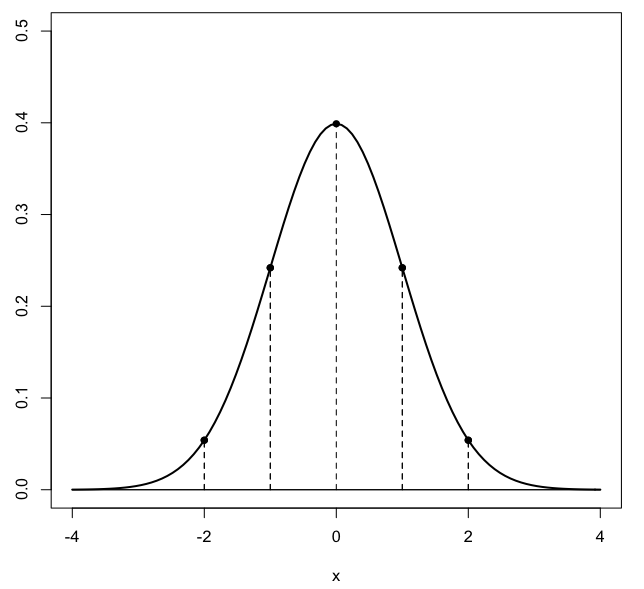
\includegraphics [scale=0.4] {gauss3.png} \end{center}

%break
\title{Nullspace of a matrix}
\date{}

\begin{document}
\maketitle
\Large

Let's consider two vectors in R2.
\[ \mathbf{a} = \ <3,4> \ = 
\begin{bmatrix}
3 \\
4
\end{bmatrix}
\]
\[ \mathbf{b} = \ <-3,1> \ = 
\begin{bmatrix}
-3 \\
\ \ 1
\end{bmatrix}
\]
We can see from a plot that these two vectors are obviously not pointing in the same direction.
\begin{center} 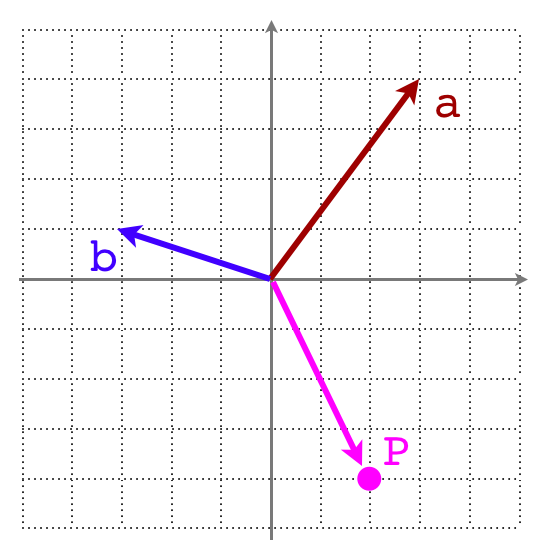
\includegraphics [scale=0.4] {null1.png} \end{center}
We say that $\mathbf{a}$ is not a multiple (or a linear combination) of $\mathbf{b}$, because there is no constant $k$ such that $k \times \mathbf{a} = \mathbf{b}$.  Now consider a point $P$ anywhere in R2, say $(2,-4)$.

We can construct a linear combination of $\mathbf{a}$ and $\mathbf{b}$ that reaches this $P$ or any other point.  Simply place one of the vectors at the origin and move along it (perhaps in a negative direction), and place the second vector at $P$ and move along it, and find where the two lines meet.
\begin{center} 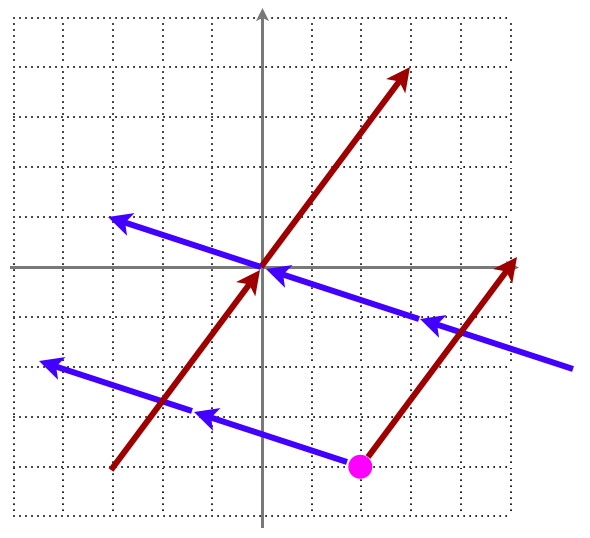
\includegraphics [scale=0.4] {null2.png} \end{center}
Call the coordinates of the point where the lines cross $x$ and $y$. There are actually two possibilities depending on which vector we choose for each role. Suppose we move in the reverse direction from the origin along $\mathbf{a}$ (in quadrant III) and from $P$ to the left along $\mathbf{b}$. From the point-slope equation we know that:
\[ (0-y)/(0-x) = 4/3 \]
\[ y = \frac{4}{3}x \]
because the slope of $\mathbf{a}$ is $4/3$, and
\[ (P_y-y)/(P_x-x) = -\frac{1}{3} \]
because the slope of $\mathbf{b}$ is $-1/3$.  Plugging in $P=(2,-4)$, we have
\[ \frac{-4 - y}{ \ \ 2 - x} = -\frac{1}{3} \]
\[ 12 + 3y =  2 - x  \]
\[ x = - 10 - 3y =  -10 - 3 \ \frac{4}{3}x = -10 - 4x\]
\[ x = -2 \]
\[ y = -\frac{8}{3} \]
The other solution is symmetrical (we're dealing with a parallelogram). We would need to go $+2$ across and $+8/3$ up from $P$ to reach $x, y = (4, -4/3)$.
Suppose we want to know the actual multipliers for $\mathbf{a}$ and $\mathbf{b}$, i.e. the fraction of the length of $a$ and $b$ that we travel along each vector.
From the figure, we can estimate that the values will be about $-0.7$ and $-1.25$.
\begin{center} 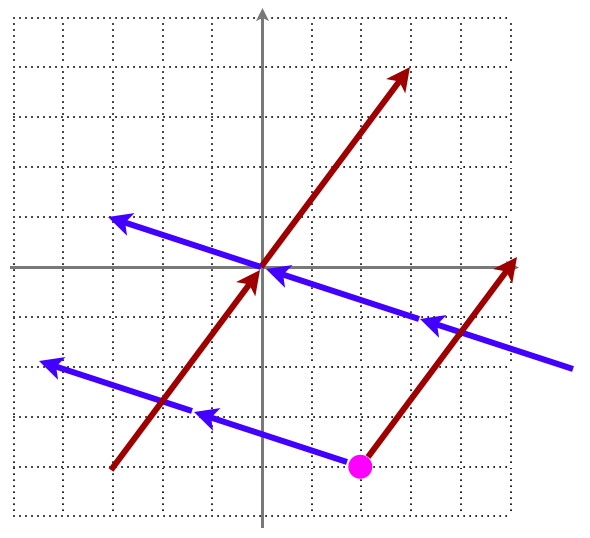
\includegraphics [scale=0.4] {null2.png} \end{center}
Call these multipliers $u$ and $v$.  In matrix language, we arrange our two vectors $\mathbf{a}$ and $\mathbf{b}$ in a matrix like this
\[ M = 
\begin{bmatrix}
\mathbf{a} \mathbf{b}
\end{bmatrix}
=
\begin{bmatrix}
3 & -3 \\
4 & \ \ 1 
\end{bmatrix}
\]
We set up a multiplication
\[ \begin{bmatrix}
3 & -3 \\
4 & \ \ 1 
\end{bmatrix}
\begin{bmatrix}
u \\
v
\end{bmatrix}
=
\begin{bmatrix}
\ \ 2 \\
-4 
\end{bmatrix}
\]
One way we can solve the system (the Algebra 2 way) is to do the multiplication
\[ 3u - 3v = 2 \]
\[ 4u + v = -4 \]
Solve the second equation for $v$ and plug into the first
\[ 3u -3(-4 - 4u) = 2 \]
\[ 15u = -10 \]
\[ u = -\frac{2}{3} \]
\[ v = -4 -4(-\frac{2}{3}) = -\frac{4}{3} \]
In matrix language we would say that
\[ \begin{bmatrix}
3 & -3 \\
4 & \ \ 1 
\end{bmatrix}
\begin{bmatrix}
u \\
v
\end{bmatrix}
=
\begin{bmatrix}
3 & -3 \\
4 & \ \ 1 
\end{bmatrix}
\begin{bmatrix}
-2/3 \\
-4/3
\end{bmatrix}
=
\begin{bmatrix}
\ \ 2 \\
-4 
\end{bmatrix}
\]
Now, consider $P$ as not just a point but a vector $\mathbf{c}$.  Then our multiplication is $u$ times the first column (vector $\mathbf{a}$) + $v \times \mathbf{b}$ is equal to vector $\mathbf{c} = \ <2,-4>$.
\[ -\frac{2}{3} 
<3,4>
+
-\frac{4}{3} 
<-3,1> \ = \
<-2+4,-\frac{8}{3} -  \frac{4}{3}> \ = \
<2,-4>
\]
Since we could have chosen $P$ to be any point, $\mathbf{c}$ can be any vector in the x,y-plane and it can be constructed as a linear combination of $\mathbf{a}$ and $\mathbf{b}$:
\[ \mathbf{c} = u \ \mathbf{a} +  v \ \mathbf{b} \]
We say that $\mathbf{c}$ is in the \emph{column space} of the matrix whose columns are the vectors $\mathbf{a}$ and $\mathbf{b}$.
\[ M = 
\begin{bmatrix}
\mathbf{a} \mathbf{b}
\end{bmatrix}
=
\begin{bmatrix}
3 & -3 \\
4 & \ \ 1 
\end{bmatrix}
\]
because we can obtain $\mathbf{c}$ as a linear combination of the columns of $M$.  
\[ u\ \mathbf{a} +  v \ \mathbf{b}\ = \mathbf{c} \]
\[ M 
\begin{bmatrix}
u \\
v
\end{bmatrix}
=
\begin{bmatrix}
\mathbf{a} \mathbf{b}
\end{bmatrix}
\begin{bmatrix}
u \\
v
\end{bmatrix}
=
\mathbf{c} \]
Using just the two vectors $\mathbf{a}$ and $\mathbf{b}$, there is no linear combination that gives the zero vector except
\[ 0\ \mathbf{a} +  0 \ \mathbf{b}\ = 
\begin{bmatrix}
0 \\
0
\end{bmatrix}
= \mathbf{0}
\] 
But of course, since
\[ u\ \mathbf{a} +  v \ \mathbf{b}\ = \mathbf{c} \]
\[ u\ \mathbf{a} +  v \ \mathbf{b}\ - \mathbf{c} = \mathbf{0} \]
\[ u\ \mathbf{a} +  v \ \mathbf{b}\ + w \ \mathbf{c} = \mathbf{0} \]
($w=-1$).  
But once we add $\mathbf{c}$ to the matrix $M'$ there is a way to do it.
\[ M' = 
\begin{bmatrix}
\mathbf{a} \mathbf{b} \mathbf{c}
\end{bmatrix}
=
\begin{bmatrix}
3 & -3 & \ \ 2 \\
4 & \ \ 1 & -4
\end{bmatrix}
\]
\[ 
\begin{bmatrix}
3 & -3 & \ \ 2 \\
4 & \ \ 1 & -4
\end{bmatrix}
\begin{bmatrix}
u \\
v \\
w
\end{bmatrix}
=
\begin{bmatrix}
3 & -3 & \ \ 2 \\
4 & \ \ 1 & -4
\end{bmatrix}
\begin{bmatrix}
-2/3 \\
-4/3 \\
- 1
\end{bmatrix}
= 
\begin{bmatrix}
0 \\
0 \\
0
\end{bmatrix}
\]
The combination $u = -2/3, v = -4/3, w = -1$ solves this equation and brings us back to zero.  This new vector, call it $\mathbf{x}$ 
\[ \mathbf{x} = 
\begin{bmatrix}
u \\
v \\
w
\end{bmatrix}
=
\begin{bmatrix}
-2/3 \\
-4/3 \\
- 1
\end{bmatrix}
\]
is said to be in the \emph{nullspace} of $M'$ because $M' \mathbf{x} = \mathbf{0}$.

For any matrix $M$, if there exists a non-zero solution $\mathbf{x}$ to
\[ M \mathbf{x} = \mathbf{0} \]
it's the same thing as saying we can find $u,v,w$ such that
\[ u\ \mathbf{a} +  v \ \mathbf{b}\ + w \ \mathbf{c} = \mathbf{0} \]
and then among the consequences are these two:  that the columns of $M$ are not linearly independent
\[ u\ \mathbf{a} +  v \ \mathbf{b}\ = - w \ \mathbf{c} \]
and the determinant of $M$ is equal to $0$, because we can "zero out" one of the columns of $M$.


\end{document}  